\section*{Въпроси}

\begin{questions}

  \question[10] Кое от следните не е правилно разделяне на мрежата
  \texttt{10.0.0.0/22} на три подмрежи?

  \begin{choices}
    \choice \texttt{10.0.0.0/24}, \texttt{10.0.1.0/24}, \texttt{10.0.2.0/23}
    \CorrectChoice \texttt{10.0.0.0/23}, \texttt{10.0.2.0/24}, \texttt{10.0.3.0/24}
    \choice \texttt{10.0.0.0/24}, \texttt{10.0.1.0/23}, \texttt{10.0.3.0/24}
  \end{choices}

  \question[6] На кой слой от седемслойния OSI модел или петслойния BSD модел
  работят маршрутизаторите?
  \begin{oneparchoices}
    \choice 1
    \choice 2
    \CorrectChoice 3
    \choice 4
    \choice 5
  \end{oneparchoices}

  \question[6] На кой слой от седемслойния OSI модел или петслойния BSD модел
  работят комутаторите (\foreignlanguage{english}{switches})
  \begin{oneparchoices}
    \choice 1
    \CorrectChoice 2
    \choice 3
    \choice 4
    \choice 5
  \end{oneparchoices}

  \question[6] Маршрутната таблица съдържа: (изберете един верен отговор)
  \begin{choices}
    \choice съответствия между IP и MAC адреси
    \choice списък с всички MAC адреси на системи, с които хостът е разменял
    рамки
    \CorrectChoice списък на пътищата към IP мрежите, с които хостът може да
    разменя IP пакети
    \choice списък на всички IP aдреси, с които хостът е разменял IP пакети
  \end{choices}

  \question[6] RIP и OSPF са протоколи за:
  \begin{choices}
    \choice Намиране на съответствието между IP aдрес и MAC aдерес.
    \choice Диагностика на мрежови проблеми.
    \choice Комуникация между автономни системи (AS).
    \CorrectChoice Размяна на маршрути.
  \end{choices}

  \question[6] BGP e:
  \begin{choices}
    \choice протокол, използван за комуникация с най-близкия комутатор в
    локалната мрежа.

    \choice IGP протокол.

    \CorrectChoice протокол за динамична маршрутизация, основно използван от
    маршрутизаторите, седящи на границата между две AS
    (\foreignlanguage{english}{border routers}).

    \choice наследник на TCP протокола.
  \end{choices}

  \question[6] UDP добавя поле за порт, чиято дължина е:
  \begin{oneparchoices}
    \CorrectChoice 8 бита.
    \choice 9 бита.
    \choice 12 бита.
    \choice 16 бита
    \choice 18 бита.
  \end{oneparchoices}

  \question[6] Полето "`\foreignlanguage{english}{destination port}"', което TCP
  и UDP въвеждат...
  \begin{choices}
    \choice съвпада с последните два октета от мрежовата маска.
    \choice се маскира със старшите три октета на MAC адреса.
    \CorrectChoice се използва за адресация на мрежовите приложения, които
    работят на крайния хост.
    \choice се използва за намиране на маршрутизатора по подразбиране.
  \end{choices}

  \question[6] Броят на валидните TCP или UDP портове е:
  \begin{oneparchoices}
    \choice 255
    \choice 256
    \choice 32768
    \CorrectChoice 65535
    \choice 262144
    \choice 4096
  \end{oneparchoices}

  \question[10] Мрежата \texttt{10.0.0.0/28} може да се раздели на най-много
  \begin{choices}
    \choice 2 подмрежи.
    \choice 3 подмрежи.
    \CorrectChoice 4 подмрежи.
    \choice Не може да се раздели на подмрежи.
  \end{choices}

  \question[10] Мрежата \texttt{10.0.0.0/24} съдържа подмрежите:
  \begin{oneparchoices}
    \choice \texttt{10.0.1.0/25}
    \choice \texttt{10.0.0.0/23}
    \choice \texttt{10.0.1.0/24}
    \CorrectChoice \texttt{10.0.0.0/25}
    \choice \texttt{10.0.2.0/25}
  \end{oneparchoices}

  \question[6] Командите "`\texttt{echo 1 > /proc/sys/net/ipv4/ip\_forward}"' и \\
  "`\texttt{sysctl -w net.ipv4.ip\_forward=1}"' под Linux:
  \begin{choices}
    \CorrectChoice активират подсистемата за маршрутизация на ядрото.
    \choice спират активния Ethernet интерфейс.
    \choice увеличават с 1 последния октет на адреса на хоста.
    \choice забраняват IPv6 протокола.
  \end{choices}

  \question[6] Ако сме на хост в мрежа \texttt{10.0.0.0/24} и знаем, че имаме
  маршрутизатор с адрес \texttt{10.0.0.1} в мрежата, с коя команда добавяме
  маршрут до мрежа \texttt{192.168.0.0/24}?
  \begin{choices}
    \choice \texttt{route add -net 192.168.0.0/24 gw 10.0.0.0}
    \CorrectChoice \texttt{route add -net 192.168.0.0/24 gw 10.0.0.1}
    \choice \texttt{route add -net 192.168.0.0/24 gw 10.255.255.255}
    \choice \texttt{route add -net 192.168.0.0/24 gw 10.0.0.255}
    \choice \texttt{route add -net 192.168.255.255/24 gw 10.0.0.1}
  \end{choices}

  \question[6] Коя от следните мрежи не следва да бъде маршрутизируема в Интернет?
  \begin{choices}
    \choice \texttt{1.0.0.0/22}
    \choice \texttt{2.0.0.0/24}
    \CorrectChoice \texttt{172.16.3.0/24}
    \choice \texttt{200.0.0.0/22}
    \choice \texttt{192.169.0.0/16}
  \end{choices}

  \question[6] Кои от следните твърдения са верни за IP? (Изберете три отговора)
  \begin{choices}
    \CorrectChoice Интернет протоколът (IP) е пример за протокол от мрежовия
    слой на OSI модела.

    \CorrectChoice В момента за комуникация в Интернет се използват основно две
    версии на IP – IP версия 4 и IP версия 6.

    \choice IP е пример за протокол от транспортния слой на OSI модела и
    предоставя надеждна комуникация.

    \CorrectChoice IP не гарантира, че пакетите ще бъдат доставени в реда, в
    който са изпратени или изобщо.
  \end{choices}

  \question[6] Кое от следните твърдения е вярно за IP?
  \begin{choices}
    \choice IP датаграмите (\foreignlanguage{english}{datagram}) съдържат поле
    "`\texttt{\foreignlanguage{english}{hop-count}}"', към чиято стойност бива
    добавена единица всеки път, когато датаграмата премине през маршрутизатор
    (\foreignlanguage{english}{router}).

    \choice IP датаграмите съдържат
    \texttt{\foreignlanguage{english}{time-to-live}} поле, което се състои от
    списък на всички маршрутизатори, през които е преминал пакетът, за да може
    крайният хост да установи дали пакета е бил затворен в цикъл.

    \CorrectChoice IP датаграмите съдържат целочислено поле, на базата на чиято
    стойност се открива и прекратява препредаването им в безкраен цикъл.

    \choice \texttt{\foreignlanguage{english}{time-to-live}} полето пренася
    данни от транспортния слой.
  \end{choices}

  \question[6] Кои от следните са директни последствия от изборите, направени
  при проектирането на TCP? (Изберете два верни отговора)
  \begin{choices}
    \choice TCP е самодостатъчен и наличната адресна информация в TCP хедъра
    позволява при провеждане на комуникация да не се използва мрежовия слой или
    който и да е друг по-нисък слой.

    \choice TCP не изисква състоянието на връзката да бъде установено преди
    участниците в комуникацията да започнат да обменят данни.

    \CorrectChoice TCP ще изпрати отново липсващите данни, дори ако приложението
    не може да ги използва -- например при Интернет телефонията -- закъснели
    данни може да пристигнат прекалено късно, за да бъдат полезни.

    \CorrectChoice TCP спестява нуждата в приложението да бъдат имплементирани
    механизми за преизпращане на неполучени данни или преподреждане на данни,
    получени в неправилен ред данни.

    \choice TCP може да функционира, само ако слоят под него също гарантира
    надеждност и последователност на данните.
  \end{choices}

  \question[6] TCP използва three-way handshake, защото: (Изберете два верни
  отговора)

  \begin{choices}

    \CorrectChoice При TCP, крайните точки пазят информация за състоянието на
    комуникацията в двете посоки и ръкостискането позволява това състояние да
    бъде инициализирано и синхронизирано.

    \choice Традицията налага, когато двама души се запознаят, да си стиснат
    ръцете.

    \choice Вместо тристранно, TCP може да използва двустранно
    ръкостискане. Третата стъпка е въведена единствено, за да се предотврати
    подслушването на данните.

    \CorrectChoice TCP установява поток от данни и в двете посоки. Тристранното
    ръкостискане позволява двата потока от данни да бъдат установени и потвърдени.
  \end{choices}

  \question[7] Кои от следните твърдения, относно UDP, са верни? (Изберете три
  верни отговора)

  \begin{choices}
    \choice Никое приложение не би искало да използва UDP, защото не предоставя
    надежден транспорт на данните.

    \CorrectChoice UDP често се използва за разпръскване
    \foreignlanguage{english}{broadcast} на данни, защото не изисква
    установяването на състояние за всеки получател на данните.

    \CorrectChoice За кратка комуникация от вид "`заявка-отговор"', използвана
    например при DNS, се предпочита използването на UDP, за да се избегнат
    служебните разходи (\foreignlanguage{english}{overhead}) на TCP.

    \CorrectChoice UDP е подходящ за приложения, които не се нуждаят
    задължително от надежден транспорт на данни
    (пр. \foreignlanguage{english}{voice-over-IP}, онлайн игри).
  \end{choices}

  \question[6] Кои от следните са следствия от енкапсулацията на данните?
  (Изберете два верни отговора)

  \begin{choices}
    \CorrectChoice Запазване на разделението на слоевете на архитектурата.

    \choice Изпращане на по-голямо количество данни по мрежата.

    \CorrectChoice Опростяване на имплементацията на слоевете на архитектурата.

    \choice Защита от злонамерени атаки.
  \end{choices}

  \question[6] Кой слой се намира между физическия и мрежовия слой?
  \begin{oneparchoices}
    \choice Сесийният.

    \choice Транспортният.

    \CorrectChoice Каналният (\foreignlanguage{english}{data-link}).

    \choice Презентационният.
  \end{oneparchoices}

  \question[6] Всеки маршрутизатор (\foreignlanguage{english}{router}) може да
  бъде свързан най-много с два други маршрутизатора.
  \begin{oneparchoices}
    \choice Вярно.
    \CorrectChoice Грешно.
  \end{oneparchoices}

  \question[6] Целта на маршрута по подразбиране
  (\foreignlanguage{english}{default route}) е да покаже накъде трябва да бъдат
  пренасочени пакетите, чиято дестинация не съвпада с никой друг запис в
  маршрутната таблица.
  \begin{oneparchoices}
    \CorrectChoice Вярно.
    \choice Грешно.
  \end{oneparchoices}

  \question[6] Сегменти с вдигнат \texttt{FIN} флаг се изпращат при създаване на
  TCP връзка.
  \begin{oneparchoices}
    \choice Вярно.
    \CorrectChoice Грешно.
  \end{oneparchoices}

  \question[10] Кои от следните адреси са част от мрежата \texttt{192.13.128.0} с
  мрежова маска \texttt{255.255.128.0}?
  \begin{choices}
    \CorrectChoice 192.13.128.0
    \CorrectChoice 192.13.255.1
    \CorrectChoice 192.13.255.64
    \choice 192.13.0.0
    \choice 192.13.64.2
    \CorrectChoice 192.13.192.255
  \end{choices}

  \question[6] Вярно ли е, че мрежа с маска "`\texttt{/8}"' съдържа
  $2^{24}$ адреса, които могат да бъдат зачислени на хостове?
  \begin{oneparchoices}
    \choice Вярно.
    \CorrectChoice Грешно.
  \end{oneparchoices}


  \question[6] Вярно ли е, че мрежа с маска "`\texttt{/8}"' съдържа точно
  $2^8$ адреса, които могат да бъдат зачислени на хостове?
  \begin{oneparchoices}
    \choice Вярно.
    \CorrectChoice Грешно.
  \end{oneparchoices}

  \question[7] Посочете вярното твърдение, относно NAT.
  \begin{choices}
    \choice Невъзможно е хостовете, намиращи се зад NAT да инициират връзки с Интернет.
    \choice Замисълът на NAT е да прочита всички пакети и да пропуска само безопасните.
    \CorrectChoice Възможно е да се използва верига от повече от един
    маршрутизатор, извършващ NAT.
  \end{choices}

  \question[7] Външен хост се опитва да създаде TCP връзка с хост, слушащ на
  порт \texttt{5577} зад NAT (\foreignlanguage{english}{Masquerade} или
  \foreignlanguage{english}{Port-address translation}). Към кой порт на
  маршрутизатора, извършващ динамичен NAT, трябва да адресира TCP сегментите си
  външния хост?

  \begin{choices}
    \choice Трябва да ги адресира към порт 5577. NAT автоматично ще препрати
    сегментите към вътрешния хост на базата на таблицата си.

    \choice Може да ги адресира към всеки порт на маршрутизатора, но първите 16
    бита на съдържанието, енкапсулирано в TCP сегмента, трябва да съдържат
    \texttt{5577}. Ако вътрешният хост е зад NAT, тези 16 бита винаги ще бъдат
    използвани за определяне на вътрешния порт.

    \CorrectChoice В общия случай не може да се даде гаранция, че сегментите ще
    бъдат маршрутизирани до вътрешния хост.
  \end{choices}

  \begin{center}
    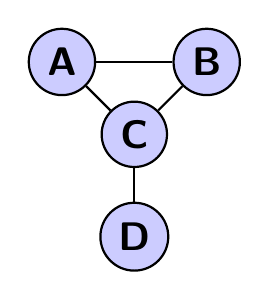
\begin{tikzpicture}[auto,node distance=1.3cm,
      thick,main node/.style={circle,fill=blue!20,draw,font=\sffamily\Large\bfseries}]


      \node[main node] (3) {C};
      \node[main node] (1) [above left of=3] {A};
      \node[main node] (2) [above right of=3] {B};
      \node[main node] (4) [below of=3] {D};


      \path[every node/.style={font=\sffamily\small}]
        (1) edge node {} (3)
            edge node {} (2)
        (2) edge node {} (3)
        (3) edge node {} (4);
    \end{tikzpicture}
  \end{center}

  \question[7] На графиката отгоре са изобразени четири маршрутизатора, които са
  конфигурирани за динамична маршрутизация с RIP. Ако не са имплементирани
  оптимизации за алгоритъма на RIP, какво ще бъде разстоянието между A и
  D след една стъпка от схождането на мрежата. (Приемете, че маршрутизаторите са
  били изключени до този момент)

  \begin{oneparchoices}
    \choice 1
    \CorrectChoice безкрайност
    \choice 3
    \choice 2
  \end{oneparchoices}

\end{questions}

%%% Local Variables: 
%%% mode: latex
%%% TeX-master: "test"
%%% TeX-PDF-mode: t
%%% End: 
